% !TeX spellcheck = en_US
\color{fontcolor}

\begin{frame}
	Recommended reading:
	\begin{itemize}
		\item Lectures 24, 25, 27 in \cite{TreBau}
		\item Sections I.6 in \cite{StrangData}
		\item Sections 6.1, 6.2, 6.4 in \cite{StrangLA_intro}	
		\item Kapitel 7 in \cite{Rannacher}
	\end{itemize}
	
	%	\bibliographystyle{plain}
	~\\~\\
	Literature:\\
	\bibliography{../information/literature.bib}
\end{frame}
\begin{frame}
\Section{Eigenvalues: Theory and Algorithms}	
\Subsection{Introduction}
\Hide{
\begin{example}[Illustration in 2d: Part 1]\label{ex:eigvals-Illustration-2d-1}
	~\\
		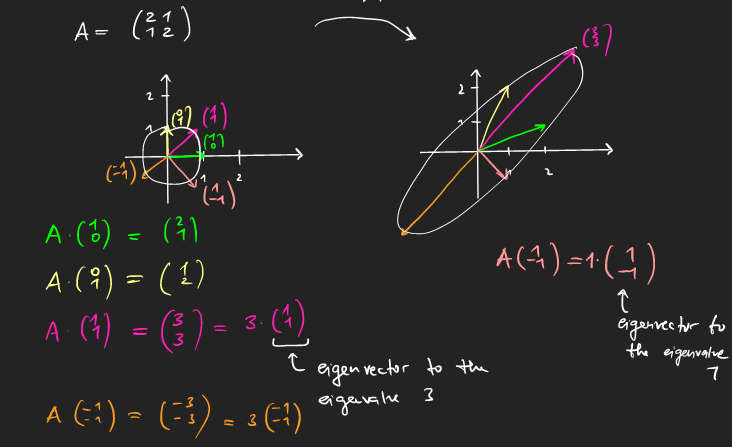
\includegraphics[width=0.94\textwidth]{eigenvalues_example.png}
\end{example}
}
\end{frame}




% EIGENVALUES
\begin{frame}
\Subsection{Eigenvalues and Eigendecompositon}
\begin{defi}[Eigenvalues and -vectors]\label{def:eigvals}
	Let $A\in\F^{n\times n}$ be a matrix. A number $\lambda\in \C$ is called an \textbf{\emph{eigenvalue}} of $A$, if 
	$$\exists v\in \F^n, v\neq 0\colon~Av=\lambda v.$$ In that case, $v$ is called an \textbf{\emph{eigenvector}} and $(\lambda, v)$ an \textbf{\textit{eigenpair}}. The set of all eigenvalues is denoted by
	$$\sigma(A):=\{\lambda\in \C\colon \lambda \text{ is eigenvalue of }A\}$$ and called the \textbf{\emph{spectrum of $A$}}.
\end{defi}

\begin{itemize}
	\item[1)] Assume we knew an eigenvalue $\lambda$:\\
		\Hide{
	Then we find a corresponding eigenvector by solving the linear equation $$(A - \lambda I_n)v = 0 $$
	Observation: 
	\begin{center}
		$v$ eigenvector ~~~$\Rightarrow$~~~ $\alpha v$ eigenvector $\forall \alpha\in \F$
	\end{center}

~\\
	 We often normalize the eigenvector by $\frac{v}{\|v\|_2}$. } 
    \vspace{0.5cm}
	\item[2)]  Assume we had an eigenvector $v$:\\
		\Hide{
		Then the corresponding eigenvalue is uniquely determined by the so-called \textit{Rayleigh-Quotient} $$ \lambda =  \frac{v^TAv}{v^Tv}$$}
\end{itemize}
\end{frame}



% DETERMINANTS AND EIGENVALUES
\begin{frame}
\textbf{The determinant and eigenvalues}\\~\\
Let $A\in \F^{n \times n}$. Then:~\\
\Hide{
\begin{itemize}
	\item[1)] \textbf{Relation between the determinant and eigenvalues:}
	\begin{align*}
	\lambda\in\C \text{~eigenvalue of~} A ~~& \Leftrightarrow~~\exists v\neq 0\colon Av = \lambda v    ~~\Leftrightarrow ~~\exists v\neq 0\colon~(A-\lambda I_n)v = 0 \\[0.25cm]
	~~& \Leftrightarrow~~\exists v\neq 0\colon~v \in \ker(A-\lambda I_n)  ~~ \Leftrightarrow~~ (A-\lambda I_n) \text{~not injective} \\[0.25cm]
	~~& \Leftrightarrow~~ (A-\lambda I_n) \notin \text{GL}(n,\mathbb{F}) ~~\Leftrightarrow ~~\det (A-\lambda I_n) =0
	\end{align*}
	\item[2)] \textbf{Implication:}\\
	By invoking the Laplace formula (see Def.\ref{def:Laplace-formula}) for the determinant we can show that the function $$\lambda \mapsto \chi_A(\lambda) := \det (A-\lambda I_n)$$ is a \textbf{polynomial of degree} $\leq n$. Thus, we can state:
	$$\textit{\textbf{ The eigenvalues of $A$ are the roots of the polynomial $\chi_A(\lambda)$}}.$$
	The fundamental theorem of algebra then assures the existence of eigenvalues (at most $n$ distinct ones).~\\
	~\\
	Definition: The polynomial $\chi_A(\lambda)$ is called \textbf{\color{defgruen}characteristic polynomial of $A$}.
\end{itemize}
}
\end{frame}


% ILLUSTRATION in 2d
\begin{frame}
\Hide{
\begin{example}[Illustration in 2d: Part 2] \label{ex:eigvals-Illustration-2d-2}~\\
	Let us consider the $(2\times 2)$ matrix 
	$$
	A = \begin{pmatrix}
	2&1\\1&2
	\end{pmatrix}
	$$
	from Example \ref{ex:eigvals-Illustration-2d-1} above.
	
	\begin{itemize}
		\item We compute its eigenvalues by solving the following root finding problem:
			\begin{align*}
		&0=\chi_A(\lambda)=\text{det}(A-\lambda I)=~\text{det}\left(\begin{pmatrix}
		2-\lambda&1\\1&2-\lambda
		\end{pmatrix}\right) = (2-\lambda)^2-1\\
		&\Leftrightarrow~~\lambda\in\{3,1\}=:\{\lambda_1,\lambda_2\}=\sigma(A)
		\end{align*}
		\item Now that we have the eigenvalues we can find corresponding eigenvectors by solving the following homogeneous linear systems:\\
\begin{itemize}
	\item 		For $\lambda_1 = 3$:
		
		$$(A-\lambda_1 I)v^1=0~~\Leftrightarrow~~\begin{pmatrix}
		-1&1\\1&-1
		\end{pmatrix}v^1=0~~\Rightarrow~~v_1^1-v_2^1=0$$
		Thus, the set of all eigenvectors corresponding to the eigenvalue $\lambda_1$ is given by
	$$
		E(\lambda_1):=\{v\in\mathbb{R}^2:~Av=\lambda_1v\}~~=~~\{v\in\mathbb{R}^2:~v_1^1=v_2^1\}
		=~~\lbrace\begin{pmatrix}\alpha\\
		\alpha\end{pmatrix}\in\mathbb{R}^2:~\alpha\in\mathbb{R}\rbrace
		=~~\text{span}\left(\begin{pmatrix}1\\1\end{pmatrix}\right)
		$$
		~\\
		Sometimes it is reasonable to choose eigenvectors of length $1$, so that we normalize: $v^1 = \frac{1}{\sqrt{2}} \begin{pmatrix}1\\1\end{pmatrix}$\\~\\
\end{itemize}
	\end{itemize}


\end{example}
}
\end{frame}

\begin{frame}
	~\\
\Hide{	\begin{itemize}
		\item[] \begin{itemize}
			\item 	For $\lambda_2 = 1$:
	$$
	(A-\lambda_2 I)v^2=0~~\Leftrightarrow~~\begin{pmatrix}
	1&1\\1&1
	\end{pmatrix}v^2=0~~\Leftrightarrow~~v_1^2+v_2^2=0
	$$
	Thus, the set of all eigenvectors corresponding to the eigenvalue $\lambda_2$ is given by
	$$	
	E(\lambda_2) 
	:= \{v\in\mathbb{R}^2:~Av=\lambda_2v\}
	=\{v\in\mathbb{R}^2:~v_1^2=-v_2^2\}
	=\lbrace\begin{pmatrix} \alpha\\-\alpha\end{pmatrix}\in\mathbb{R}^2:~\alpha\in\mathbb{R}\rbrace
	=\text{span}\left(\begin{pmatrix}1\\-1\end{pmatrix}\right) $$
	~\\
	Normalization: Choose $v^2 = \frac{1}{\sqrt{2}} \begin{pmatrix}1\\-1\end{pmatrix}$\
		\end{itemize}
	\item[] ~\\~\\
	\textit{Remark:}\\ The set of all eigenvectors corresponding to the eigenvalue $\lambda \in \sigma(A)$, i.e., $$E(\lambda) = \ker(A-\lambda I) \subset \F^n$$  is called \textbf{\color{defgruen}eigenspace to the eigenvalue $\lambda$ of $A$}.
	\end{itemize}
}
\end{frame}



\begin{frame}
\begin{lemma}[Matrix and Eigenvalue Properties]\label{lem:properties_eigenvalues}~\\[-0.1cm]
	\begin{itemize}
	\item[\color{satzrot}i)]Power of a matrix: $A \in \F^{n\times n} ,~\lambda \in \sigma(A) ~~\Rightarrow~~  \lambda^k \in \sigma(A^k)~\text{for any}~k\in \N$ 
	\vspace{0.2cm}\item[\color{satzrot}ii)] Inverse matrix: $A \in GL_n(\F),~\lambda \in \sigma(A) ~~\Rightarrow~~ \lambda\neq 0,~\frac{1}{\lambda} \in \sigma(A^{-1})~$
	\vspace{0.2cm}\item[\color{satzrot}iii)]Scaling: $A \in \Fnn,~\lambda \in \sigma(A)~~\Rightarrow~~\alpha \lambda \in \sigma(\alpha A) ~~\text{for any} ~\alpha \in \F$
	\vspace{0.2cm}\item[\color{satzrot}iv)] $A \in \F^{n\times n}$hermitian $(A = A^H)$ $~~\Rightarrow~~ \sigma(A)\subset\R$.
	\vspace{0.2cm}\item[\color{satzrot}v)]  $Q \in \Fnn$ unitary ($Q^HQ=I$), $\lambda \in \sigma(Q) ~~\Rightarrow~~|\lambda|=1$
	\vspace{0.2cm}\item[\color{satzrot}vi)] $A \in \F^{n\times n}$ positive definite (semi-definite) ($x^HAx>0$ ($\geq 0$)) $~~\Leftrightarrow~~\forall \lambda \in \sigma(A)\colon~ \lambda > 0~  (\lambda \geq 0)$
	\vspace{0.2cm}\item[\color{satzrot}vii)] The eigenvalues of an upper (lower) triangular matrix are sitting on the diagonal.
	\vspace{0.2cm}\item[\color{satzrot}viii)] Similarity transformation: $A \in \Fnn, ~T \in GL_n(\F) ~~\Rightarrow~~ \sigma(A) = \sigma(T^{-1}AT)$
	\vspace{0.2cm}\item[\color{satzrot}ix)] Shifts: $A \in \Fnn,~ (\lambda, v)$ eigenpair of $A  ~~\Rightarrow~~ \forall s\in\F \colon ~ (\lambda+s, v)$ eigenpair of $A+sI$	
\end{itemize}
\end{lemma}


~\\~\\
\textbf{Attention:} The following rules do not hold in general:\\[-0.1cm]
\begin{itemize}
	\item $\lambda \in \sigma(A), \mu \in \sigma(B)~~~\nRightarrow~~~(\lambda + \mu) \in \sigma(A+B)$
	\item $\lambda \in \sigma(A), \mu \in \sigma(B)~~~\nRightarrow~~~(\lambda \cdot \mu) \in \sigma(A\cdot B)$
\end{itemize}
\end{frame}


\begin{frame}
	\begin{proof}
		Exercise. \Hide{Here, we exemplary prove viii):
		}
	\end{proof}
\end{frame}






%DIAGONALIZING
\begin{frame}
\textbf{Diagonalizing a matrix}\\
\Hide{
	~\\
Let us consider a matrix
$A\in\mathbb{F}^{n\times n}$ with eigenpairs $(\lambda_i,v_i)\in\F \times\mathbb{F}^n$, so that 
$$Av_i = \lambda_i v_i,~~~\text{for}~1\leq i\leq n.$$ 
Using matrix notation this can be written as
\begin{align*}
A\cdot\underbrace{\begin{pmatrix}
|&|&~&|\\v_1&v_2&\cdots&v_n\\|&|&~&|
\end{pmatrix}}_{=:V\in\mathbb{F}^{n\times n}}
&=\begin{pmatrix}
|&|&~&|\\\lambda_1 v_1&\lambda_2 v_2&\cdots&\lambda_n v_n\\|&|&~&|
\end{pmatrix}
=\begin{pmatrix}
|&~&|\\v_1&\cdots&v_n\\|&~&|
\end{pmatrix}
\underbrace{\begin{pmatrix}
\lambda_1&~&0\\~&\ddots&~\\0&~&\lambda_n
\end{pmatrix}}_{=:\Lambda\in\mathbb{F}^{n\times n}}
\end{align*}
which is equivalent to
$$A V = V \Lambda .$$
~\\
If $V$ is invertible (note that this is not necessarily the case!), then we can rearrange this into the following decomposition
$$
V^{-1}AV=\Lambda~~\Leftrightarrow~~A=V\Lambda V^{-1}.
$$
~\\
One central question arises:  When is $V$ invertible?
}
\end{frame}

\begin{frame}
Let us first revisit the example from above (see Examples \ref{ex:eigvals-Illustration-2d-1} and \ref{ex:eigvals-Illustration-2d-2})\\~\\
\Hide{~\\
\begin{example}[Illustration in 2d: Part 3] \label{ex:eigvals-Illustration-2d-3}~\\
Let us again consider the \textit{real symmetric} matrix
$$A=\begin{pmatrix}
2&1\\1&2
\end{pmatrix},$$
with eigenpairs
$$\lambda_1=3,~v_1=\frac{1}{\sqrt{2}}\begin{pmatrix}1\\1\end{pmatrix},~~~~
\lambda_2=1,~v_2=\frac{1}{\sqrt{2}}\begin{pmatrix}1\\-1\end{pmatrix}.$$
~\\
Assembling the normalized eigenvectors into the matrix $V$ yields
$$
V=\frac{1}{\sqrt{2}}
\begin{pmatrix}
1&1\\1&-1
\end{pmatrix}.$$
~\\
Since for the columns we have
\begin{align*}
~\begin{pmatrix}1\\1\end{pmatrix}^T\begin{pmatrix}1\\-1\end{pmatrix}=1-1=0
\end{align*}
and by construction
$$
\|v_1\|_2=\frac{1}{\sqrt{2}}\underbrace{\lVert\begin{pmatrix}1\\1\end{pmatrix}\rVert}_{=\sqrt{2}}=1,~~~\text{and similarly}~~ \|v_2\|_2 = 1,
$$
we find that $V$ is orthogonal and thus in particular invertible.
\end{example}
}
\end{frame}



% EXAMPLE
\only<article>{
\begin{ex}
	 
	Symmetric matrix: $A = \begin{bmatrix}
	4 & 2 \\
	2 & 1
	\end{bmatrix}$\\
	\begin{align*}
	p(\lambda) &= \alpha_0 + \alpha_1\lambda + \alpha_2 \lambda^2 = 2-2\lambda + \lambda^2\\
	&= (4\cdot 1-2\cdot 2)-(4+1)\lambda +\lambda^2 \\
	&=-5\lambda + \lambda ^2 \\
	&=(-5+\lambda)\lambda \\
	&\Rightarrow \lambda_1 = 0, \lambda_2 = 5 \;\;\text{(eigenvalues)}\\
	\end{align*}
	eigenvectors:
	\begin{itemize} 
		\item[$v1$)] \begin{align*}
		&Av=\lambda v \Leftrightarrow (A-\lambda I)v=0\\[10pt]
		&\begin{bmatrix}
		4 & 2 \\
		2 & 1
		\end{bmatrix} \begin{bmatrix}
		x_1 \\
		x_2
		\end{bmatrix} = \begin{bmatrix}
		0 \\
		0
		\end{bmatrix} \underrightarrow{REF} \begin{bmatrix}
		4 & 2 \\
		0 & 0
		\end{bmatrix} \begin{bmatrix}
		x_1 \\
		x_2
		\end{bmatrix} = \begin{bmatrix}
		0 \\
		0
		\end{bmatrix}\\[10pt]
		&4x_1 + 2x_2 = 0 \Rightarrow 2x_1 + x_2 =0 \Rightarrow x_2=-2x_1\\[10pt]
		&v_1 = r \left( \begin{array}{c}
		1 \\
		-2 
		\end{array} \right), r\in \mathbb{R} \;\; \text{normed eigv:~} \overline{v_1} = \frac{1}{\sqrt{5}}\left(\begin{array}{c}
		1 \\
		-2 
		\end{array} \right)
		\end{align*}\\
		\item[$v2$)] \begin{align*}
		&A - \lambda_2 I = \begin{bmatrix}
		4 & 2 \\
		2 & 1
		\end{bmatrix} - 5\begin{bmatrix}
		1 & 0 \\
		0 & 1
		\end{bmatrix} = \begin{bmatrix}
		-1 & 2 \\
		2 & -4
		\end{bmatrix}\\
		&\begin{bmatrix}
		-1 & 2 \\
		2 & -4
		\end{bmatrix}\begin{bmatrix}
		x_1 \\
		x_2
		\end{bmatrix} = \begin{bmatrix}
		0 \\
		0
		\end{bmatrix} \Rightarrow (REF) \begin{bmatrix}
		-1 & 2 \\
		0 & 0
		\end{bmatrix} \begin{bmatrix}
		x_1 \\
		x_2
		\end{bmatrix} = \begin{bmatrix}
		0 \\
		0
		\end{bmatrix}\\
		&\Rightarrow x_1 = 2x_2 \;\;\Rightarrow\;\; v_2 = r \left( \begin{array}{c}
		2 \\
		1
		\end{array} \right) \Rightarrow \bar{v_2} = \frac{1}{\sqrt{5}}\left(\begin{array}{c}
		2 \\
		1 
		\end{array} \right)
		\end{align*}
	\end{itemize}	
	Test that they are orthogonal:\\
	\begin{align*}
	M &:= [\bar{v_1},\bar{v_2}] = \frac{1}{\sqrt{5}} \begin{bmatrix}
	1 & 2 \\
	-2 & 1
	\end{bmatrix} \;\; \text{is orthogonal} \\
	M^\top M &= \frac{1}{\sqrt{5}} \begin{bmatrix}
	1 & -2 \\
	2 & 1
	\end{bmatrix}, \frac{1}{\sqrt{5}} \begin{bmatrix}
	1 & 2 \\
	-2 & 1
	\end{bmatrix} = \frac{1}{\sqrt{5}} \begin{bmatrix}
	1 & -2 \\
	2 & 1
	\end{bmatrix} \begin{bmatrix}
	1 & 2 \\
	-2 & 1
	\end{bmatrix} = \begin{bmatrix}
	1 & 0 \\
	0 & 1
	\end{bmatrix}
	\end{align*}
\end{ex}
}






%%%%%%%%%%%%%%%%%%%%%%%%%%%%%%%%%%%%%%%%%%%%%%%%%%%%%%%%%%%
% PYTHON EXAMPLE with heat equation
\only<article>{
\begin{minipage}[c]{0.35\textwidth}
	{\bf Eigenvalues of the symmetric \\
		matrix:}
	
	\medskip
	{\small
		$A=
		-\begin{pmatrix} 
		-2F & F\\
		F & -2F & F \\
		& \ddots & \ddots & \ddots\\
		&        &  F     & -2F    
		\end{pmatrix}
		$
	}
	
	for varying grid sizes ordered in size. $x$-axis is just the current number of the ordered eigenvalues, i.e., the bullet points are the
	pairs $(\frac{i}{\tt Nx}, \lambda_i)$.
	
	\begin{tikzpicture}
	\node[inner sep=0pt] (dina0) at (0,0)
	{\includegraphics[width=\textwidth]{LocalFolder/LocalMedia/5_heat1D-eigs.png}};
	\end{tikzpicture}
	
\end{minipage}
\begin{minipage}[c]{0.05\textwidth}
	\
\end{minipage}
\begin{minipage}[c]{0.6\textwidth}
%	\lstinputlisting{LocalFolder/LocalMedia/python_examples/5_heat1D-eig.py}
\end{minipage}
%%%%%
\begin{minipage}[c]{0.4\textwidth}
	{\bf Selected eigenvectors:}
	
	\begin{tikzpicture}
	\node[inner sep=0pt] (dina0) at (0,0)
	{\includegraphics[width=\textwidth]{LocalFolder/LocalMedia/5_eigv_30.png}};
	\end{tikzpicture}
	(Note: ``frequency$_i$''$=\sqrt{\lambda_i}$)
\end{minipage}
\begin{minipage}[c]{0.05\textwidth}
	~
\end{minipage}
\begin{minipage}[c]{0.55\textwidth}
%	\lstinputlisting[firstline=4]{LocalFolder/LocalMedia/python_examples/5_heat1D-eigv.py}
\end{minipage}
}
%%%%%%%%%%%%%%%%%%%%%%%%%%%%%%%%%%%%%%%%%%%%%%%%%%%%%%%%%%%
%%%%%%%%%%%%%%%%%%%%%%%%%%%%%%%%%%%%%%%%%%%%%%%%%%%%%%%%%%%%

\begin{frame}
In the previous Example \ref{ex:eigvals-Illustration-2d-3} the matrix $V$ of eigenvectors turned out to be orthogonal. The next theorem states, that this is true for any real symmetric matrix.
\begin{theo}[Eigendecomposition of real symmetric matrices]\label{theo:eigen_sym}
	For any symmetric matrix $A\in\R^{n\times n}$, there is an orthogonal matrix $Q\in\R^{n\times n}$ (i.e., $Q^\top Q=I$) such that
	$$
	Q^\top AQ=\begin{pmatrix}
	\lambda_1 \\
	&\lambda_2\\
	&&\ddots\\
	&&&\lambda_n
	\end{pmatrix} =: \text{diag}(\lambda_1,\ldots,\lambda_n)
	\text{~~(=~\textit{diagonal matrix})}
	$$
	and $\lambda_i\in\R,i \in \{1,\ldots, n\}$, are the eigenvalues of $A$. The columns of $Q$ are the normalized eigenvectors.
\end{theo}
\begin{proof}
	In the exercises we will prove this statement for the special case that the matrix has $n$ distinct eigenvalues. The general proof is rather technical and can be found in any standard textbook.
\end{proof}
~\\
$\rightarrow$ \textbf{Thus:} ``knowing the eigenpairs = knowing the matrix''\\
~\\~\\~\\
An immediate consequence of Theorem \ref{theo:eigen_sym} is this: \vspace{-0.3cm}
\begin{corollary} A symmetric matrix $A\in\R^{n\times n}$ is invertible, if and only if all its eigenvalues are nonzero.
\end{corollary}

\end{frame}
 
\begin{frame}
~\\
\Hide{
Let us again continue our example:
\begin{example}[Illustration in 2d: Part 4] \label{ex:eigvals-Illustration-2d-4}~\\
For the \textit{symmetric} matrix
$$A=\begin{pmatrix}
2&1\\1&2
\end{pmatrix},$$
with eigenpairs
$$\lambda_1=3,~v_1=\frac{1}{\sqrt{2}}\begin{pmatrix}1\\1\end{pmatrix},~~~~
\lambda_2=1,~v_2=\frac{1}{\sqrt{2}}\begin{pmatrix}1\\-1\end{pmatrix}$$
let us set
$$Q:= V=\frac{1}{\sqrt{2}}\begin{pmatrix}
1&1\\1&-1
\end{pmatrix}  ~~~ \text{and} ~~
 \Lambda:=\begin{pmatrix}
3&0\\0&1
\end{pmatrix}.$$
~\\
Indeed, we can verify
\begin{align*}
A=Q\Lambda Q^T &=\frac{1}{2}\underbrace{
	\begin{pmatrix}
	1&1\\1&-1
	\end{pmatrix}
	\underbrace{\begin{pmatrix}
		3&0\\0&1
		\end{pmatrix}
		\begin{pmatrix}
		1&1\\1&-1
		\end{pmatrix}
	}_{=\begin{pmatrix}3&3\\1&-1\end{pmatrix}}
}_{=\begin{pmatrix}4&2\\2&4\end{pmatrix}}\\
&=\begin{pmatrix}
2&1\\1&2
\end{pmatrix}.
\end{align*}
~\\
\end{example}
}
\end{frame} 


\begin{frame}
~\\
Geometry of the eigendecomposition:~\\~\\
\Hide{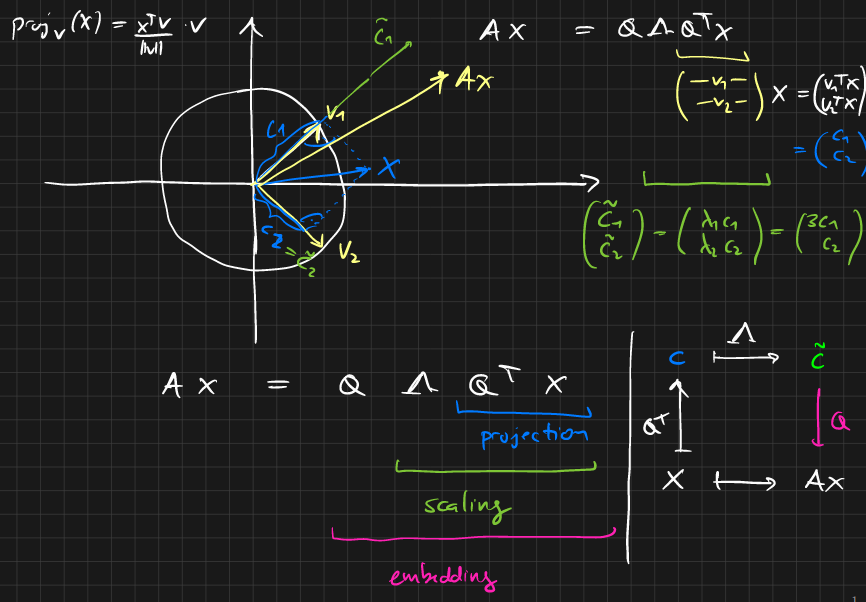
\includegraphics[width=0.9\textwidth]{projection_scaling_embedding.png}}
\end{frame}




 


\begin{frame}
\Subsection{Eigenvalue Algorithms: Solving the eigenvalue problem}
~\\
\textbf{Aim:} Solving the \textit{\textbf{eigenvalue problem}} defined by
\begin{center}
	\textit{Given $A \in \Fnn$, find eigenpairs $(\lambda_i, v_i)$ so that, for all $i=1,\ldots,n$,
		$$v_i \neq 0 ~~\text{and}~~Av_i = \lambda_i v_i .$$}  
\end{center}
Sometimes we are only interested in a few eigenpairs $(\lambda_i, v_i)$ (for example the one with largest eigenvalue in magnitude). In this case we call it a \textit{partial} eigenvalue problem.
~\\~\\~\\
\textbf{Overview}\\~\\
\begin{itemize}
	\item[\bfseries 1.]\textbf{A first naive approach: Direct method}\\
	$\rightarrow$ only feasible for very small matrices: $n\in\{2,3,4\}$ \\~\\
	\item[\bfseries 2.]\textbf{Partial eigenvalue problem: Simple iterative methods} (here: The Power Method)\\
	$\rightarrow$ determine a \textit{single} eigenpair	\\~\\
	\item[\bfseries 3.] \textbf{A second advanced approach: General iterative method} (here: The $QR$ algorithm)  \\
	$\rightarrow$ determine \textit{all} eigenpairs
\end{itemize}
\end{frame}






\begin{frame}
\Subsubsection{A first naive approach: Direct method}
~\\
~\\~\\
\textbf{ Recipe:}
	 \begin{itemize}
	\item[a)] Eigenvalues:\\
	 Solving \textbf{\color{cyan}root finding problem} for the characteristic polynomial
	$$\chi_A(\lambda) := \det (A-\lambda I) = 0 $$  yields the eigenvalues $\lambda_i$.
	\vspace{0.6cm}\item[b)] Eigenvectors:\\
	Solving the homogeneous \textbf{\color{orange}linear system}
	$$(A - \lambda_i I)v_i = 0$$ 
	for each distinct  $\lambda_i$, gives the corresponding eigenvectors $v_i$ (or more precisely, eigenspaces).
\end{itemize}
\end{frame}


\begin{frame}
	\textbf{Example:} $n = 2$\\
	Consider a general $(2 \times 2)$-matrix $A=\begin{pmatrix} a&b\\c&d\end{pmatrix}$.
	\begin{itemize}
		\item[a)] \textbf{\color{cyan}Root finding problem}:\\
		 Above, we have derived a closed formula for the determinant of a $(2 \times 2)$-matrix, which applied to $A-\lambda I$ gives
		\[
		0=\chi_A(\lambda)=\det(A -\lambda I)=\det\left(\begin{pmatrix} a-\lambda&b\\c&d-\lambda\end{pmatrix}\right) = (a-\lambda)(d-\lambda) - cb = \lambda^2 - (a+d)\lambda + (ad-cb)
		\]
		$$\rightarrow \lambda_{1/2} =   \frac{a+d}{2} \pm \sqrt{\left(\frac{a+d}{2}\right)^2 -(ad-cb) }.$$
		\item[b)] \textbf{\color{orange}Linear system}:\\ We then have to solve 
		$$\begin{pmatrix}
		a-\lambda_i&b\\c&d-\lambda_i
		\end{pmatrix} \begin{pmatrix}
		v_1^i\\v_2^i
		\end{pmatrix}~~~\text{for}~~~i=1,2 .$$
		$$\rightarrow  v^1, v^2$$
	\end{itemize}
	~\\
	Note: For $n=3$ we can proceed similarly by applying the rule of Sarrus in step a).
	
	\only<article>{
		$\bullet$ $n=2$:\\
		The eigenvalues $\lambda$ of the matrix $A=\begin{pmatrix}
		 
		 a&b\\c&d\end{pmatrix}$ satisfy
		\[
		0=\chi_A(\lambda)=\det(A -\lambda I)=\det\left(\begin{pmatrix} a-\lambda&b\\c&d-\lambda\end{pmatrix}\right) = (a-\lambda)(d-\lambda) - cb
		\]
		$\rightarrow$ compare to the formula presented on Sheet 06
		~\\~\\
		$\bullet$ $n=3$:\\
		Similarly, the eigenvalues $\lambda$ of $A = \left(\begin{bmatrix}
		\textcolor{cyan}{a_{11}} & \textcolor{orange}{a_{12}} & \textcolor{cyan}{a_{13}}\\
		\textcolor{orange}{a_{21}} & \textcolor{cyan}{a_{22}} & \textcolor{orange}{a_{23}}\\
		\textcolor{cyan}{a_{31}} & \textcolor{orange}{a_{32}} & \textcolor{cyan}{a_{33}}
		\end{bmatrix}\right)$ are determined by
		$$0=\chi_A(\lambda)=\det(A -\lambda I)=\det\left(\begin{bmatrix}
		\textcolor{cyan}{a_{11}} -\lambda& \textcolor{orange}{a_{12}} & \textcolor{cyan}{a_{13}}\\
		\textcolor{orange}{a_{21}} & \textcolor{cyan}{a_{22}} -\lambda& \textcolor{orange}{a_{23}}\\
		\textcolor{cyan}{a_{31}} & \textcolor{orange}{a_{32}} & \textcolor{cyan}{a_{33}}-\lambda
		\end{bmatrix}\right)$$
		$\rightarrow$ we can apply Sarrus rule} 
\end{frame}

\begin{frame}

	~\\~\\
	\textbf{Problem:}\\~\\
	In practice, for general, potentially very large, matrices the root finding problem is infeasible, because: \\
	\begin{center}
		$A$ with large dimension $n$ $~~\Rightarrow~~$ $\chi_A$ high polynomial degree $~~\Rightarrow~~$ high risk of rounding errors
	\end{center}
	~\\
	{\footnotesize See for example:\\
	\url{https://en.wikipedia.org/wiki/Root-finding_algorithms\#Roots\_of\_polynomials}
	}
	~\\
	~\\~\\
	\textbf{Abel–Ruffini theorem} (see related discussion in \cite[Theorem 25.1]{TreBau}):\\ \textit{There are no ``closed formulas'' for the roots of general polynomials with degree higher than $4$.}
	~\\~\\~\\
	\textbf{As a consequence}: \begin{center}
		We cannot solve the eigenvalue problem in finitely many steps.\\ Instead, any eigenvalue algorithm has to be iterative!
	\end{center}
	\end{frame}



 
% POWER METHOD
\begin{frame}
\Subsubsection{Simple Iterative Method: The Power Iteration}
$\rightarrow$ basis for PageRank algorithm from Google and the WTF algorithm from Twitter~\\~\\
%\textbf{Idea:} 

 \Hide{\begin{example}[Illustration in 2d: Part 5] \label{ex:eigvals-Illustration-2d-5}~\\
 		Again, let us consider $A=\begin{pmatrix}
	2&1\\1&2
	\end{pmatrix},~\lambda_1=3,~v_1=\frac{1}{\sqrt{2}}\begin{pmatrix}1\\1\end{pmatrix},~\lambda_2=1,~v_2=\frac{1}{\sqrt{2}}\begin{pmatrix}1\\-1\end{pmatrix}$.\\
Let us successively apply the matrix $A$ to an initial guess $w^0 \in\R^n$:\\
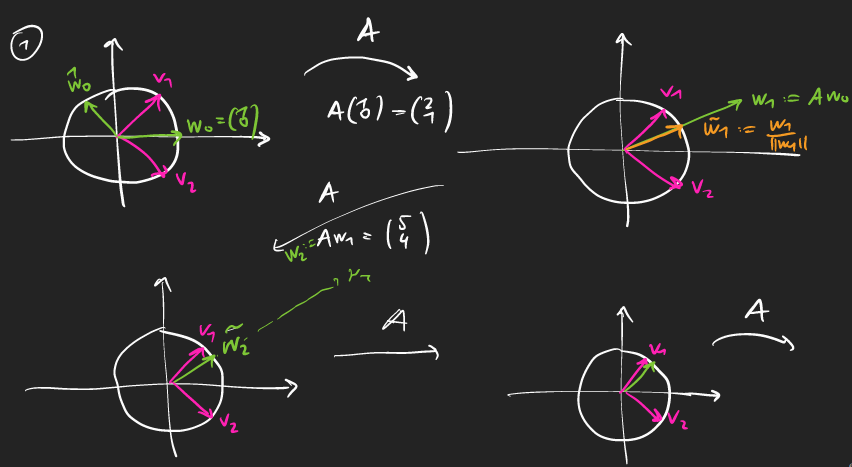
\includegraphics[width=0.8\textwidth]{power_method_idea.png}\\
Note: The normalization step can be performed with respect to any norm.
 	\end{example}
}
\end{frame}




\begin{frame}
%We find the following convergence result.
 \begin{theorem}[Convergence of power iteration]
 Let $A\in\R^{n\times n}$ be a matrix with eigenvalues $\lambda_i$ for $i \in \{1,\ldots, n\}$ which satisfy
 $
 |\lambda_1|>|\lambda_2|\ge\ldots\ge|\lambda_n|
 $
and whose eigenvectors form a basis of $\R^n$. Also, let the sequence of vectors $\{w^k\}_{k=0}^\infty$ be defined by the so-called \textbf{power iteration}
 \[
 w^{k+1}:=\frac{Aw^k}{\|Aw^k\|_p}\, ,\ k\ge 0, p\geq 1,~~\text{with}~~ \ w^0 \text{ such that } (v^1, w^0)_2 \neq 0,
 \]
 where $v^1$ is the normalized (i.e., $\|v^1\|_p=1$) eigenvector corresponding to $\lambda_1$. Then, for ${k\to\infty}$, we find $w^k\mathop{\longrightarrow} \pm v^1$ and also the so-called \emph{Rayleigh quotients} $$\mu_k:=\frac{(w^k,Aw^k)_2}{(w^k,w^k)_2}\mathop{\longrightarrow}\lambda_1.$$
 \end{theorem}\small
\begin{proof}
	See, e.g., \cite[Satz 7.3]{Rannacher} or \cite[Theorem 27.1 ]{TreBau}. 
\Hide{The idea: Let $v^i \in \R^n$ be the corresponding eigenvectors. Then we can write the initial guess as linear combination
	$w^0 = \sum_{j=1}^n \mu_j v^j (\mu_1 \neq 0),$
	so that with $c_k := \frac{1}{\|Aw^k\|_p}$ we find
	$$w^{k}  =c_k A^k w^0 = c_k\sum_{j=1}^n \mu_j A^k v^j= c_k\sum_{j=1}^n \mu_j \lambda_j^k v^j= c_k\lambda_1^k\left( \mu_1 v^1 + \sum_{j=2}^n \mu_j\left(\frac{ \lambda_j}{ \lambda_1}\right)^k v^j\right).$$
	The fractions $\left(\tfrac{ \lambda_j}{ \lambda_1}\right)^k$ vanish as $k \to \infty$ and the limit vector is in $\text{span}(v^1)$. Since $\|w^k\|_p=\|v^1\|_p=1$ the result follows.
	}
\end{proof}
\textit{Remark:} 
\begin{itemize}
 	\item A variant of this approach is given by the so-called \textbf{inverse power method}, which can estimate any eigenpair, assumed a good initial guess for the eigenvalue is available.
 	\item The assumption on the eigenvectors is satisfied, e.g., for real symmetric matrices (see Theorem \ref{theo:eigen_sym})
 	\item From the proof idea one finds that the convergence speed is determined by the fraction $\left(\tfrac{ \lambda_2}{ \lambda_1}\right)^k$ (potentially very slow).
\end{itemize}
\end{frame}




\begin{frame}
\Subsubsection{A second advanced approach: General iterative method}
~\\
 \textbf{Recall:} (Lemma \ref{lem:properties_eigenvalues})
\begin{itemize}
	\item[a)] \textbf{\color{yellow}Similar matrices} have the same eigenvalues: $$\sigma(A) = \sigma(T^{-1}AT) ~~~\text{for}~~~T\in GL_n(\F).$$
	\item[b)] \textbf{\color{codegreen}Simple matrices}: Eigenvalues of an upper triangular matrix $U$ (e.g., a diagonal matrix) are found on its diagonal, i.e.,
	$$\sigma(U) = \{u_{11},\ldots, u_{nn} \} .$$
\end{itemize}
~\\
\textbf{Recipe:}
  \begin{itemize}
	\item[a)] Iteratively applying \textbf{\color{yellow}similarity transformations} $T_k \in GL_n(\F)$ to $A=: A_0$ thereby producing a sequence
	$$A_{k} = T_k^{-1} A_{k-1} T_k. $$
	\vspace{0.15cm}\item[b)] Choose $T_k$ so that this sequence converges to a \textbf{\color{codegreen}simple matrix} (triangular or even diagonal)
	$$ A_\infty :=\lim_{k\to\infty} A_k  .$$
\end{itemize}
~\\
$\rightarrow$ \textbf{Question:} Choice of the $T_k$'s?
\end{frame}


\begin{frame}
	~\\
\textbf{Requirements} on the transformations $T_k$:
		\begin{itemize}
			\item[1.] easily constructed from $A_{k-1}$
			\item[2.] easy to invert (e.g., orthogonal matrix)
			\item[3.] $(A_k)_k$ converges to something simple
	\end{itemize}
~\\~\\
	 \textbf{One Implementation:}
	 \begin{itemize}
	 	\item[a)] The \textbf{\color{yellow}$QR$-Algorithmn} defines such transformations $T_k$ through\\ \vspace{-0.15cm}
	 	\begin{minipage}{0.3\textwidth}
	 		~
	 	\end{minipage}
	 	\begin{minipage}[c]{0.6\textwidth}
	 		\vspace{0.2cm}
	 		\begin{tabbing}
	 			\qquad \= \qquad \= \qquad \kill
	 			$A_0=A$\\
	 			\textbf{for} $k=1,\ldots ,\infty$\ : \\[0.3em]
	 			\> $Q_{k}R_{k}:=A_{k-1}$ \\[0.3em]
	 			\> $A_{k}:=R_{k}Q_{k}$ 
	 		\end{tabbing}	 
	 	\end{minipage}
	 	~\\~\\~\\ \vspace{0.2cm}
	 	\Hide{
	 	Thus, inserting the first equation ${\color{cyan}R_{k}} =Q_{k}^TA_{k-1} $ into the second gives
	 	$$A_{k} ={\color{cyan}R_{k}}Q_{k}= Q_{k}^TA_{k-1}Q_{k}= Q_{k}^T  Q_{k-1}^TA_{k-2}Q_{k-1}Q_{k} = \cdots = \overline{Q}_{k}^T A \overline{Q}_{k},$$
	 	 where $$\overline{Q}_k := Q_1 \cdot Q_2 \cdots Q_{k-1}\cdot Q_{k}$$
	 	Here: $T_k = Q_{k-1}$, where $Q_{k-1}$ is derived from the $QR$ decomposition of $A_{k-1}$.
	 }
	 \end{itemize}
\end{frame}




% SIMULTANEAOUS POWER ITERATION
%\begin{frame}
%\textbf{Recall:} Power iteration
%\vspace{-0.7cm}
%\begin{align*}
%q_{k+1} := \frac{A q^k}{\|A q^k\|_2} ~~~&~~~\xrightarrow[k\to \infty]{}  v_1\\
%q_{k+1} := q_k^T A q_k ~~~&~~~\xrightarrow[k\to \infty]{}  \lambda_1
%\end{align*}
%{\bf Idea:} Simultaneous power iteration for a whole orthogonal matrix instead of a single vector, like ``$Q_{k+1}=AQ_k$''. 
%
%{\bf Problem:} $AQ_k$ is no longer an orthogonal matrix in general, but, we can orthogonalize it.
%This idea yields the \textbf{simultaneous iteration (SI)}:\\
%\begin{minipage}{0.3\textwidth}
%	~
%\end{minipage}
%\begin{minipage}[c]{0.6\textwidth}
%	\vspace{0.2cm}
%	\begin{tabbing}
%		\qquad \= \qquad \= \qquad \kill
%		$\overline{Q}_0:=I$\\
%		\textbf{for} $k=0,\ldots ,\infty$\ : \\[0.3em]
%		\> $\overline{Q}_{k+1}R_{k+1}:=A  \overline{Q}_k$   \\[0.3em] 
%		\> $A_{k+1}:=  \overline{Q}_{k+1}^TA\overline{Q}_{k+1}$
%	\end{tabbing}	 
%\end{minipage}
%\end{frame}

 
%\begin{frame}
%which is shown in {\color{cyan}\url{https://arxiv.org/abs/1105.1185}} to be equivalent to 
%In fact, it is shown that\\[-0.16cm]
%\begin{itemize}
%	\item[i)] The $\overline{Q}_k$ from the (SI) are the products of the $Q_{k}$ from the (QRI), i.e.,
%	$$\overline{Q}_k = Q_1 \cdot Q_2 \cdots Q_{k-1}\cdot Q_{k} $$
%	\item[ii)] This implies that the iterates $A_k$ are the same in both iterations:
%	$$ A^{QRI}_{k}=R_{k}Q_{k}= (Q_{k}^TQ_{k})\cdot  R_{k}Q_{k} = Q_{k}^TA_{k-1}Q_{k} = \overline{Q}_{k}^T A \overline{Q}_{k} = A^{SI}_{k} $$
%\end{itemize}
%Since the $\overline{Q}_k$ are orthogonal, we find that all iterates $A_k = \overline{Q}_{k}^T A \overline{Q}_{k}$ are \emph{\color{defgruen} orthogonally similar} to $A$. In particular, all $A_k$ and their limit $A_\infty := \lim_{k\to \infty}A_k$ have the \textit{same} eigenvalues as $A$ (see exercises).\\~\\
%\textbf{Good news:} In many cases $A_\infty$ is (quasi) upper triangular, so that we can finds its eigenvalues on the diagonal.
%\end{frame}
% 



\begin{frame}
\begin{itemize}
	\item[b)] We find: $A_{k} = \overline{Q}_k^T A\overline{Q}_k  \xrightarrow[k\to \infty]{} U$, where $U$ is {\color{codegreen}\textbf{(quasi) upper triangular}}; given as follows:
\begin{theorem}[$QR$ Algorithm]
Consider a matrix $A\in\R^{n\times n}$ with distinct eigenvalues $\lambda_i$ for $i=1,\ldots,n$, i.e.,
$
|\lambda_1|>|\lambda_2|>\ldots>|\lambda_n|
$. Then the iterates $A_k\in\R^{n\times n}$ produced by the $QR$ algorithm converge to the diagonal matrix $\Lambda := \text{diag}(\lambda_1, \ldots, \lambda_n)$ which consists of the eigenvalues of $A$, i.e., 
$$\lim_{k\to \infty} A_k = \Lambda. $$~\\
\end{theorem}
\begin{proof}
	See, e.g., \cite[Satz 7.8]{Rannacher}.
\end{proof}
~\\~\\
Finally: \textbf{What about the eigenvectors?}\\~\\
One can further show that similar to the power iteration, we find that the columns of $$\overline{Q}_\infty := \lim_{k\to \infty}\overline{Q}_k$$ are normalized eigenvectors of $A$.
\end{itemize}
\end{frame}


 
%
\begin{frame}
\Subsubsection{In Practice: Combined Iterative Methods}
\textbf{Problems:}\\
\begin{itemize}
	\item $QR$ decomposition for general and very large matrices too expensive
	\item Exact Schur complement is not reached in finitely many steps ( = many $QR$ decompositions needed)
\end{itemize}
\textbf{However:}
\begin{itemize}
	\item Any matrix can be \textbf{\color{magenta}reduced} to a Hessenberg matrix (= simple matrix) in \textit{finitely many} steps
	\item $QR$ decomposition for this type of matrix is cheap
\end{itemize}
~\\
This leads to:\\
\textbf{(3) A third state-of-the-art approach: Combined iterative methods}
\begin{itemize}
	\item[a)] \textbf{\color{magenta}Similarity transformation via reduction} (e.g., Householder, Wilkinson, Givens) to something simple such as Hessenberg or even tridiagonal\\ \textit{($\rightarrow$ finite steps)}
	\vspace{0.25cm}\item[b)] \textbf{\color{yellow} Similarity transformation via iterative method}  (e.g., $QR$ or $LR$ algorithm)\\ \textit{($\rightarrow$ potentially infinitely many steps)}\\\vspace{0.2cm}
	Standard: $QR$ Algorithm (with performance optimized modifications (shifts etc...))\\	
	\vspace{0.25cm}\item[c)] Determine eigenvalues from the limiting \textbf{\color{codegreen}simple matrix} (and eigenvectors from the similarity transformations).
\end{itemize}
~\\
Common combination in practice: (a) Householder reflection + (b) $QR$ algorithm
~\\
$\rightarrow$ Works pretty well for matrices up to 1 mio. columns $n \approx 10^6$\\
$\rightarrow$ for larger matrices one needs to develop problem-tailored structure exploiting methods 


\end{frame}



%%%%%%%%%%%%%%%%%%%%%
% for elomath:
% EXAMPLE: PageRank
%%%%%%%%%%%%%%%%%%%%%

%%%%%%%%%%%%%%%%%%%
% Next time (Wise 22/23): put in blue info text from exercise on power method!
%%%%%%%%%%%%%%%
\elomath{
	\begin{frame}
		\Subsection{Example: The PageRank Algorithm from Google}
		~\\~\\~\\
		\begin{minipage}[c]{0.99\textwidth}
			%	Potential Web Structure:
\begin{center}
				\begin{tikzpicture}[->,>=stealth',shorten >=1pt,auto,node distance=1.5cm,
			semithick]
			\tikzstyle{every state}=[fill=red,draw=none,text=white]	
			\node[state,fill=cyan] (A)                   {$1$};
			\node[state,scale=2.2] (B)    [right of=A]               {$2$};
			\node[state,fill=yellow,scale=1.8] (C)    [right of=B]    {\color{black}$3$};
			\node[state,fill=green] (D)    [below of=A]               {\color{black}$4$};
			\node[state,fill=brown] (E)    [below left of =C]               {$5$};
			\node[state,fill=green] (F)    [below of=C]               {\color{black}$6$};
			\node[state,fill=purple,scale=0.7] (G)    [below of=D]               {$7$};
			\node[state,fill=purple,scale=0.7] (H)    [right of=G]               {$8$};
			\node[state,fill=purple,scale=0.7] (I)    [right of=H]               {$9$};
			\node[state,fill=purple,scale=0.7] (J)    [right of=I]               {$10$};
			\node[state,fill=purple,scale=0.7] (K)    [right of=J]               {$11$};	
			\path (B) edge [bend left=15pt]  (C)
			(C) edge [bend left=15pt]  (B);
			\path (D) edge   (A)
			(D) edge   (B);
			\path (E) edge   (D)
			(E) edge (B);
			\path (F) edge [bend left=20pt]  (E)
			(E) edge [bend left]  (F)
			(E) edge  (B);
			\path (G) edge   (B)
			(G) edge [bend left=5pt] (E);
			\path (H) edge   (B)
			(H) edge (E);
			\path (I) edge   (B)
			(I) edge [bend right=5pt](E);
			\path (J) edge [bend right=5pt](E);
			\path (K) edge [bend left=2pt](E);	
			\end{tikzpicture}
\end{center}
		\end{minipage}
		~\\~\\~\\
		\begin{minipage}[c]{0.99\textwidth}
			
			\textbf{Aim:} Rank search enginge results according to the \textit{``importance''} of the web pages.\\
			
			\textbf{1998:} For this purpose, Larry Page and Sergei Brin develop the PageRank algorithm as the basis of the 
			\raisebox{-0.25\baselineskip}{
\includegraphics[width=1.2cm]{7_Google.png}} empire.\\ 
			
			\textbf{Assumption:} \textit{``important''} means more links from other (important) web pages.\\
		\end{minipage}
	~\\~\\~\\~\\
	\color{orange}
	$\rightarrow$ More details on the sheet and in the video.
	\end{frame}

}

%
%	%
%	\begin{frame}
%		~\\~\\
%		\begin{minipage}[c]{0.99\textwidth}
%	%	Potential Web Structure:
%	\begin{center}
%		\begin{tikzpicture}[->,>=stealth',shorten >=1pt,auto,node distance=1.5cm,
%		semithick]
%		\tikzstyle{every state}=[fill=red,draw=none,text=white]	
%		\node[state,fill=cyan] (A)                   {$1$};
%		\node[state,scale=2.2] (B)    [right of=A]               {$2$};
%		\node[state,fill=yellow,scale=1.8] (C)    [right of=B]    {\color{black}$3$};
%		\node[state,fill=green] (D)    [below of=A]               {\color{black}$4$};
%		\node[state,fill=brown] (E)    [below left of =C]               {$5$};
%		\node[state,fill=green] (F)    [below of=C]               {\color{black}$6$};
%		\node[state,fill=purple,scale=0.7] (G)    [below of=D]               {$7$};
%		\node[state,fill=purple,scale=0.7] (H)    [right of=G]               {$8$};
%		\node[state,fill=purple,scale=0.7] (I)    [right of=H]               {$9$};
%		\node[state,fill=purple,scale=0.7] (J)    [right of=I]               {$10$};
%		\node[state,fill=purple,scale=0.7] (K)    [right of=J]               {$11$};	
%		\path (B) edge [bend left=15pt]  (C)
%		(C) edge [bend left=15pt]  (B);
%		\path (D) edge   (A)
%		(D) edge   (B);
%		\path (E) edge   (D)
%		(E) edge (B);
%		\path (F) edge [bend left=20pt]  (E)
%		(E) edge [bend left]  (F)
%		(E) edge  (B);
%		\path (G) edge   (B)
%		(G) edge [bend left=5pt] (E);
%		\path (H) edge   (B)
%		(H) edge (E);
%		\path (I) edge   (B)
%		(I) edge [bend right=5pt](E);
%		\path (J) edge [bend right=5pt](E);
%		\path (K) edge [bend left=2pt](E);	
%		\end{tikzpicture}
%	\end{center}
%		\end{minipage}
%		~\\~\\~\\~\\
%		{\bf Idea:} A random surfer moves as follows through the web structure:
%		\begin{itemize}
%			\item[(1)] with probability $\alpha \in (0,1)$: Follows the link structure (with equal preferences to outgoing links)
%			\item[(2)] with probability $(1-\alpha)$: Teleports to a random page (with equal probability) to prevent stranding in deadlocks
%			\item[$\rightarrow$] Pages, where the random surfer is more likely to appear based on the web's structure are considered more important. 
%		\end{itemize}
%		\Hide{
%			this movement is a process evolving over time:\\
%			- we need an initial state: $x_0$, saying with probability $x_0^i$ located at webpage $i$\\
%			- moving around from time step to time step is defined by (1) and (2)\\
%			- infinitely large time horizon: does this process reach a steady-state, where there is ``no visible'' movement anymore? that is the mass is distributed in such a way, that the movments are balanced --> equilibrium state! this then is considered being the page rank\\
%			$\alpha$ is damping factor}
%	\end{frame}
%
%	% P1: MOVEMENT via (1)
%	\begin{frame}
%		\begin{center}
%			\begin{minipage}[c]{0.5\textwidth}
%				%	Potential Web Structure:
%				\begin{tikzpicture}[->,>=stealth',shorten >=1pt,auto,node distance=1.9cm,	semithick]
%				\tikzstyle{every state}=[fill=red,draw=none,text=white]	
%				\node[state,fill=cyan] (A)                   {$1$};
%				\node[state,scale=2.2] (B)    [right of=A]               {$2$};
%				\node[state,fill=yellow,scale=1.8] (C)    [right of=B]    {\color{black}$3$};
%				\node[state,fill=green] (D)    [below of=A]               {\color{black}$4$};
%				\node[state,fill=brown] (E)    [below left of =C]               {$5$};
%				\node[state,fill=green] (F)    [below of=C]               {\color{black}$6$};
%				\node[state,fill=purple,scale=0.7] (G)    [below of=D]               {$7$};
%				\node[state,fill=purple,scale=0.7] (H)    [right of=G]               {$8$};
%				\node[state,fill=purple,scale=0.7] (I)    [right of=H]               {$9$};
%				\node[state,fill=purple,scale=0.7] (J)    [right of=I]               {$10$};
%				\node[state,fill=purple,scale=0.7] (K)    [right of=J]               {$11$};	
%				\path (B) edge [bend left=15pt]  (C)
%				(C) edge [bend left=15pt]  (B);
%				\path (D) edge   (A)
%				(D) edge   (B);
%				\path (E) edge   (D)
%				(E) edge (B);
%				\path (F) edge [bend left=20pt]  (E)
%				(E) edge [bend left]  (F)
%				(E) edge  (B);
%				\path (G) edge   (B)
%				(G) edge [bend left=5pt] (E);
%				\path (H) edge   (B)
%				(H) edge (E);
%				\path (I) edge   (B)
%				(I) edge [bend right=5pt](E);
%				\path (J) edge [bend right=5pt](E);
%				\path (K) edge [bend left=2pt](E);	
%				\end{tikzpicture}
%			\end{minipage}
%		\end{center}
%				\begin{itemize}
%			\item Let $n$ (here $11$) be the number of web pages and $e := (1,\ldots,1)^T$ 
%			\item Let $x^0 = (x^0_1, \ldots, x_n^0)$ be the initial distribution ($e^Tx_0 =1$) for the random surfer
%			\item Let us define the following matrices:
%		\end{itemize}
% \vspace*{0.3cm}
%		$$P_1={ 
%			\left(  \begin{tabular}{cccccccccccc}
%			~ & 1    & 2   & 3    & 4    & 5    & 6 & 7     & 8   & 9  & 10   & 11    \\
%			1 & 1    &~     &  ~   & 1/2  &    ~ & ~ & ~     &  ~  &  ~   & ~ &    ~  \\
%			2 & ~    & ~    &  1   & 1/2  & 1/3  &   & 1/2   & 1/2 & 1/2 &   &    \\
%			3 & ~    & 1    &  ~   &      &      &   &       &     &     &   &    \\
%			4 & ~    &  ~   & ~    &      &  1/3 &   &       &     &     &   &  \\  
%			5 & ~    &  ~   & ~    &      &      & 1 & 1/2   & 1/2 & 1/2 & 1 & 1 \\  
%			6 & ~    &  ~   &  ~   &      & 1/3  &   &       &     &     &   &  \\  
%			7 & ~    & ~    &  ~   &      &      &   &       &     &     &   &  \\  
%			8 &~     & ~    &  ~   &      &      &   &       &     &     &   &  \\  
%			9 & ~    &  ~   &  ~   &      &      &   &       &     &     &   &  \\  
%			10 & ~    &  ~   & ~    &      &      &   &       &     &     &   &  \\  
%			11 & ~    &  ~   & ~    &      &      &   &       &     &     &   &     
%			\end{tabular} \right)
%		},
%		~~~~P_2 := \frac{1}{n}ee^T= \left(\frac{1}{n}\right)_{ij}$$
%	\end{frame}
%	
%	% COLUMN STOCHASTIC MATRIX YIELDS DISTRIBUTION
%	\begin{frame}
%		\small
%		\begin{columns}[t]
%			\begin{column}{0.4\textwidth}
%				\begin{tikzpicture}[->,>=stealth',shorten >=1pt,auto,node distance=1.5cm,	semithick]
%				\tikzstyle{every state}=[fill=red,draw=none,text=white]	
%				\node[state,fill=cyan] (A)                   {$1$};
%				\node[state,scale=2.2] (B)    [right of=A]               {$2$};
%				\node[state,fill=yellow,scale=1.8] (C)    [right of=B]    {\color{black}$3$};
%				\node[state,fill=green] (D)    [below of=A]               {\color{black}$4$};
%				\node[state,fill=brown] (E)    [below left of =C]               {$5$};
%				\node[state,fill=green] (F)    [below of=C]               {\color{black}$6$};
%				\node[state,fill=purple,scale=0.7] (G)    [below of=D]               {$7$};
%				\node[state,fill=purple,scale=0.7] (H)    [right of=G]               {$8$};
%				\node[state,fill=purple,scale=0.7] (I)    [right of=H]               {$9$};
%				\node[state,fill=purple,scale=0.7] (J)    [right of=I]               {$10$};
%				\node[state,fill=purple,scale=0.7] (K)    [right of=J]               {$11$};	
%				\path (B) edge [bend left=15pt]  (C)
%				(C) edge [bend left=15pt]  (B);
%				\path (D) edge   (A)
%				(D) edge   (B);
%				\path (E) edge   (D)
%				(E) edge (B);
%				\path (F) edge [bend left=20pt]  (E)
%				(E) edge [bend left]  (F)
%				(E) edge  (B);
%				\path (G) edge   (B)
%				(G) edge [bend left=5pt] (E);
%				\path (H) edge   (B)
%				(H) edge (E);
%				\path (I) edge   (B)
%				(I) edge [bend right=5pt](E);
%				\path (J) edge [bend right=5pt](E);
%				\path (K) edge [bend left=2pt](E);	
%				\end{tikzpicture}
%			\end{column}
%			\begin{column}[t]{0.6\textwidth}
%				\vspace{-3.9cm}
%				$$P_1= { \tiny
%					\left(  \begin{tabular}{cccccccccccc}
%					~ & 1    & 2   & 3    & 4    & 5    & 6 & 7     & 8   & 9  & 10   & 11    \\
%					1 &1    &~     &  ~   & 1/2  &    ~ & ~ & ~     &  ~  &  ~   & ~ &    ~  \\
%					2 & ~    & ~    &  1   & 1/2  & 1/3  &   & 1/2   & 1/2 & 1/2 &   &    \\
%					3 & ~    & 1    &  ~   &      &      &   &       &     &     &   &    \\
%					4 & ~    &  ~   & ~    &      &  1/3 &   &       &     &     &   &  \\  
%					5 & ~    &  ~   & ~    &      &      & 1 & 1/2   & 1/2 & 1/2 & 1 & 1 \\  
%					6 & ~    &  ~   &  ~   &      & 1/3  &   &       &     &     &   &  \\  
%					7 & ~    & ~    &  ~   &      &      &   &       &     &     &   &  \\  
%					8 &~     & ~    &  ~   &      &      &   &       &     &     &   &  \\  
%					9 & ~    &  ~   &  ~   &      &      &   &       &     &     &   &  \\  
%					10 & ~    &  ~   & ~    &      &      &   &       &     &     &   &  \\  
%					11 & ~    &  ~   & ~    &      &      &   &       &     &     &   &     
%					\end{tabular} \right)
%				}$$
%				%		~T~~~P_2 := \left(\frac{1}{n}\right)_{ij}$$
%			\end{column}
%		\end{columns}
%		\begin{itemize}
%			\item[(1)] \textbf{Link structure:} Let $P_1$ be the probability matrix (column stochastic) defined by\\
%			$P_1^{ij}:=$  Probability that random surfer moves from page $j$ to page $i$ defined by the link structure
%			\item[(2)] \textbf{Jumps:}  Let $P_2$ be the probability matrix (column stochastic) defined by\\
%			$P_2^{ij} := \frac{1}{n}$= Probability that random surfer jumps from page $j$ to page $i$
%		\end{itemize}
%		The movement of the random surfer is then completely defined by the probability matrix 
%		$$P = \alpha P_1 + (1-\alpha)P_2 .$$
%		For the next time instances we obtain
%		\begin{align*}
%		x^1 &=  \alpha P_1 x^0 + (1-\alpha) P_2 x^0 = Px^0  \\
%		x^2 &=  \alpha P_1 x^1 + (1-\alpha) P_2 x^1 = Px^1 \\[0.1cm]
%		x^{k+1} &=  \alpha P_1 x^k + (1-\alpha) P_2 x^k = Px^k = P^{k+1}x_0 \\[0.1cm]
%		x^* &=  \lim_{k\to \infty} x^k =: \textbf{\textit{PageRank}} 
%		\end{align*} 
%		\textbf{Observations:} (Exercise)
%		\begin{itemize}
%			\item $P_1$, $P_2$ and thus $P$ are column stochastic (i.e., $e^TP = e^T$)
%			\item Thus, since $x^0$ prob. distribution (i.e., $e^Tx^0 = 1$), also $e^Tx^k = 1$ for all $k$ and $e^Tx^*=1$
%		\end{itemize}
%	\end{frame}
%	
%	\begin{frame}
%		\vspace{0.1cm}
%		\textbf{Question:} Does this sequence $\{x^k\}_{k \in \N}$ of vectors converge (to a steady state)?\\
%		\vspace{0.3cm}
%		One can show (\textit{later}) that this sequence converges and that its limit $x^*$ (= PageRank) solves the following equation:
%		
%		\begin{equation} \label{eq:PageRank_eigprob}
%		Px^* = 1 x^* 
%		\end{equation}
%		$$$$
%		\begin{itemize}
%			\item[$\rightarrow$]$x^*$ is an \textit{\textbf{eigenvector}} to the \textit{\textbf{eigenvalue}} $1$ of the matrix $P$.\\
%			(eigenvalue $1$ is a special case and we call the eigenvector in this case also \textit{fixed point})~\\~\\
%			\item[$\rightarrow$] Equation \eqref{eq:PageRank_eigprob} is a typical \textit{\textbf{eigenvalue problem}}.
%			~\\~\\
%			\item[$\rightarrow$]\textit{\textbf{Eigenvalue algorithms}} are developed to solve such problems. One of them is the \textit{\textbf{Power method}}, which, applied to the eigenvalue problem \eqref{eq:PageRank_eigprob}, produces precisely the sequence
%			$$x^k = P^k x^0.$$
%		\end{itemize}
%	~\\
%	 Remark: The PageRank power iteration does not need the normalization step ($\cdot 1/||Aw^k||$), since the iteration vectors are automatically bounded by the fact that the matrix involved is a stochastic matrix.
%	\end{frame}
%
%
% 
%	% Interpretation as linear system
%	\begin{frame}
%		\textbf{Remark: Interpretation as linear system}\\~\\
%		Since we interpret $x$ as a probability distribution, so that $e^\top x=1$, we obtain
%		\begin{align}
%		&x=Px = (\alpha P_1+(1-\alpha)P_2)x\label{pagerank.eig}\\
%		&=\alpha P_1x+(1-\alpha)ee^\top x=\alpha P_1x+(1-\alpha)e\quad \nonumber\\
%		\Leftrightarrow\quad &(I-\alpha P_1)x=(1-\alpha)e\label{pagerank.linsys}
%		\end{align}
%		We observe two equivalent formulations of the PageRank problem: \vspace{0.3cm}
%		\begin{itemize}
%			\item[\eqref{pagerank.eig}] As \textbf{eigenvalue problem:} Existence and uniqueness is shown by the Perron theorem (since the matrix $P$ has strictly positive entries for positive damping factors $0<\alpha<1$ the theorem yields that the maximum eigenvalue is $1$ and strictly larger than all others (see requirements for convergence of the power method).)
%			\item[\eqref{pagerank.linsys}] As \textbf{linear system:} Here we can also show that the system has a unique solution for $0<\alpha<1$, since the matrix $(I-\alpha P)$ can be classified as a \textit{diagonally dominant $M$-matrix} and is as such invertible.
%		\end{itemize}  
%	\vspace{0.3cm}
%		For large graphs, a direct solution (e.g., $LU$ decomposition) of the linear system (\ref{pagerank.linsys}) is prohibitively expensive and one has to use equation (\ref{pagerank.eig}) as a fixed point iteration in the form
%		\[
%		Px^{k}=:x^{k+1}
%		\qquad\left(
%		\Leftrightarrow x^{k+1}:=\alpha Px^{k}+(1-\alpha)e
%		\right)
%		\] 
%		which amounts to the \textbf{power method}.	\\~\\
%		Finally note that this may be applied to any graph for weighting the importance of a node according to the edge structure.
%	\end{frame}
% %end elomath
%

 


